\subsection{Caso d'uso UC5: Stampa del progetto}
\begin{figure}[h] 
	\centering 
	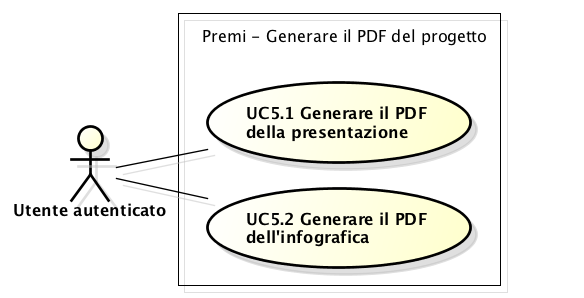
\includegraphics[scale=0.45] {img/UC5.png} 
	\caption{UC5 - Stampa del progetto} 
\end{figure}

\begin{itemize}
	\item \textbf{Attori:} Utente autenticato;
	\item \textbf{Scopo e descrizione:} L'utente ha aperto un progetto e vuole stamparne le sue parti;
	\item \textbf{Precondizione:} L'utente ha un progetto aperto e il sistema è in attesa che selezioni la funzione stampa;
	\item \textbf{Flusso principale degli eventi:}
	\begin{enumerate}
		\item L'utente seleziona la funzione di stampa della presentazione [UC5.1];
		\item L'utente seleziona le funzione di stampa dell'infografica [UC5.2];
	\end{enumerate}
	\item \textbf{Postcondizione:} Il sistema ha mandato in stampa la parte di progetto selezionata.
\end{itemize}


	\subsection{Caso d'uso UC5.1: Stampare una presentazione}
	\begin{itemize}
		\item \textbf{Attori:} Utente autenticato;
		\item \textbf{Scopo e descrizione:} L'utente ha aperto un progetto e vuole stampare la presentazione;
		\item \textbf{Precondizione:} L'utente ha un progetto aperto e il sistema è in attesa che selezioni la funzione stampa della presentazione;
		\item \textbf{Flusso principale degli eventi:}
		\begin{enumerate}
			\item L'utente seleziona la funzione stampa della presentazione [UC5.1.1];
			\item L'utente seleziona le impostazioni di stampa [UC5.1.2];
			\item L'utente conferma la stampa [UC5.1.3].
		\end{enumerate}
		\item \textbf{Postcondizione:} Il sistema ha mandato in stampa la presentazione.
	\end{itemize}
	
	\subsection{Caso d'uso UC5.1.1: Selezionare la funzione di stampa della presentazione}
	\begin{itemize}
		\item \textbf{Attori:} Utente autenticato;
		\item \textbf{Scopo e descrizione:} L'utente seleziona la funzione di stampa per stampare la presentazione;
		\item \textbf{Precondizione:} C'è una presentazione attiva e il sistema è in attesa che l'utente selezioni la funzione stampa;
		\item \textbf{Postcondizione:} Il sistema apre la finestra di dialogo per la stampa.
	\end{itemize}
	
	\subsection{Caso d'uso UC5.1.2: Selezionare le impostazioni di stampa}
	\begin{figure}[h] 
		\centering 
		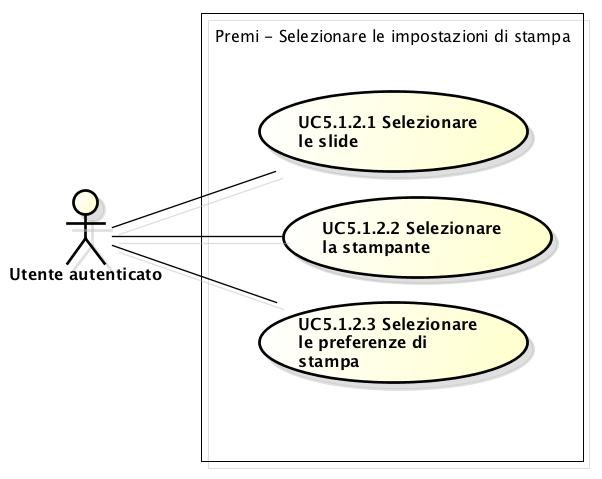
\includegraphics[scale=0.45] {img/UC5.1.2.png} 
		\caption{UC5.1.2 - Selezione delle impostazioni di stampa} 
	\end{figure}
	
	\begin{itemize}
		\item \textbf{Attori:} Utente autenticato;
		\item \textbf{Scopo e descrizione:} L'utente deve selezionare le impostazioni per la stampa della presentazione;
		\item \textbf{Precondizione:} Il sistema ha aperto la finestra di dialogo per la stampa;
		\item \textbf{Flusso principale degli eventi:}
		\begin{enumerate}
			\item L'utente seleziona quali slide stampare [UC5.1.2.1]
			\item L'utente seleziona quale stampante usare [UC5.1.2.2]
			\item L'utente seleziona le preferenze di stampa fornite dalla stampante[UC5.1.2.3]
		\end{enumerate}
		\item \textbf{Postcondizione:} Il sistema registra tutte le impostazioni selezionate dall'utente.
	\end{itemize}
	
		\subsection{Caso d'uso UC5.1.2.1: Selezionare le slide}
		\begin{itemize}
			\item \textbf{Attori:} Utente autenticato;
			\item \textbf{Scopo e descrizione:} L'utente seleziona quali slide stampare;
			\item \textbf{Precondizione:} Il sistema è in attesa che l'utente selezioni quali slide stampare;
			\item \textbf{Postcondizione:} Il sistema registra la scelta fatta dall'utente.
		\end{itemize}
		
		\subsection{Caso d'uso UC5.1.2.2: Selezionare la stampante}
		\begin{itemize}
			\item \textbf{Attori:} Utente autenticato;
			\item \textbf{Scopo e descrizione:} L'utente seleziona quale stampante installata nel sistema usare;
			\item \textbf{Precondizione:} Il sistema è in attesa che l'utente selezioni la stampante da usare;
			\item \textbf{Postcondizione:} Il sistema registra la scelta fatta dall'utente.
		\end{itemize}
		
		\subsection{Caso d'uso UC5.1.2.3: Selezionare le preferenze di stampa}
		\begin{itemize}
			\item \textbf{Attori:} Utente autenticato;
			\item \textbf{Scopo e descrizione:} L'utente seleziona le preferenze di stampa fornite dai driver della stampante stessa;
			\item \textbf{Precondizione:} Il sistema è in attesa che l'utente selezioni le preferenze da usare;
			\item \textbf{Postcondizione:} Il sistema registra la scelte fatte dall'utente.
		\end{itemize}
	
	\subsection{Caso d'uso UC5.1.3: Confermare la stampa}
	\begin{itemize}
		\item \textbf{Attori:} Utente autenticato;
		\item \textbf{Scopo e descrizione:} L'utente conferma la stampa della presentazione;
		\item \textbf{Precondizione:} L'utente ha selezionato quali slide stampare, la stampante da usare e le preferenze di stampa;
		\item \textbf{Postcondizione:} Il sistema ha mandato in stampa la presentazione.
	\end{itemize}
	
	
	\subsection{Caso d'uso UC5.2: Stampare un'infografica}
	\begin{itemize}
		\item \textbf{Attori:} Utente autenticato;
		\item \textbf{Scopo e descrizione:} L'utente ha aperto un progetto e vuole stampare l'infografica;
		\item \textbf{Precondizione:} L'utente ha un progetto aperto e il sistema è in attesa che selezioni la funzione stampa dell'infografica;
		\item \textbf{Flusso principale degli eventi:}
		\begin{enumerate}
			\item L'utente seleziona la funzione stampa dell'infografica [UC5.2.1];
			\item L'utente seleziona le impostazioni di stampa [UC5.2.2];
			\item L'utente conferma la stampa [UC5.2.3].
		\end{enumerate}
		\item \textbf{Postcondizione:} Il sistema ha mandato in stampa la presentazione.
		\end{itemize}
			
		\subsection{Caso d'uso UC5.2.1: Selezionare la funzione di stampa della presentazione}
		\begin{itemize}
			\item \textbf{Attori:} Utente autenticato;
			\item \textbf{Scopo e descrizione:} L'utente seleziona la funzione di stampa per stampare l'infografica;
			\item \textbf{Precondizione:} C'è un'infografica attiva e il sistema è in attesa che l'utente selezioni la funzione stampa;
			\item \textbf{Postcondizione:} Il sistema apre la finestra di dialogo per la stampa.
		\end{itemize}
		
		\subsection{Caso d'uso UC5.2.2: Selezionare le impostazioni di stampa}
		\begin{figure}[h] 
			\centering 
			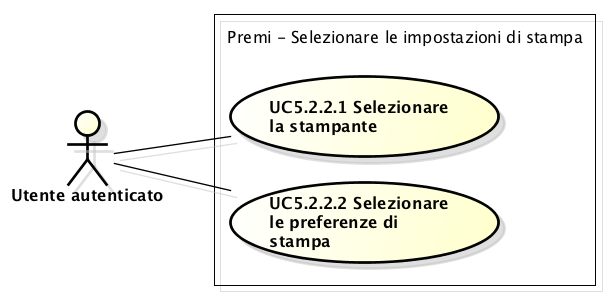
\includegraphics[scale=0.45] {img/UC5.2.2.png} 
			\caption{UC5.2.2 - Selezione delle impostazioni di stampa} 
		\end{figure}
		
		\begin{itemize}
			\item \textbf{Attori:} Utente autenticato;
			\item \textbf{Scopo e descrizione:} L'utente deve selezionare le impostazioni per la stampa dell'infografica;
			\item \textbf{Precondizione:} Il sistema ha aperto la finestra di dialogo per la stampa;
			\item \textbf{Flusso principale degli eventi:}
			\begin{enumerate}
				\item L'utente seleziona quale stampante usare [UC5.2.2.1]
				\item L'utente seleziona le preferenze di stampa fornite dalla stampante[UC5.2.2.2]
			\end{enumerate}
		\item \textbf{Postcondizione:} Il sistema registra tutte le impostazioni selezionate dall'utente.
		\end{itemize}
		
			\subsection{Caso d'uso UC5.2.2.1: Selezionare la stampante}
			\begin{itemize}
				\item \textbf{Attori:} Utente autenticato;
				\item \textbf{Scopo e descrizione:} L'utente seleziona quale stampante installata nel sistema usare;
				\item \textbf{Precondizione:} Il sistema è in attesa che l'utente selezioni la stampante da usare;
				\item \textbf{Postcondizione:} Il sistema registra la scelta fatta dall'utente.
			\end{itemize}
			
			\subsection{Caso d'uso UC5.2.2.2: Selezionare le preferenze di stampa}
			\begin{itemize}
				\item \textbf{Attori:} Utente autenticato;
				\item \textbf{Scopo e descrizione:} L'utente seleziona le preferenze di stampa fornite dai driver della stampante stessa;
				\item \textbf{Precondizione:} Il sistema è in attesa che l'utente selezioni le preferenze da usare;
				\item \textbf{Postcondizione:} Il sistema registra la scelte fatte dall'utente.
			\end{itemize}
		
		\subsection{Caso d'uso UC5.2.3: Confermare la stampa}
		\begin{itemize}
			\item \textbf{Attori:} Utente autenticato;
			\item \textbf{Scopo e descrizione:} L'utente conferma la stampa dell'infografica;
			\item \textbf{Precondizione:} L'utente ha selezionato la stampante da usare e le preferenze di stampa;
			\item \textbf{Postcondizione:} Il sistema ha mandato in stampa l'infografica.
		\end{itemize}